\documentclass{llncs}
\usepackage{tikz, graphicx}
\usetikzlibrary{arrows, arrows.meta, positioning,shadows, shapes}
\graphicspath{{./images/}}
\begin{document}
\title{Tema 2 - Retele de calculatoare}
\author{Chichirau Razvan}
\institute{Facultatea de informatica, \\ 
Universitatea Alexandru Ioan Cuza Iasi \\
\email{razvan.chichirau@info.uaic.ro}}

\maketitle

\begin{abstract}
Aceasta aplicatie a fost bazata pe cerintele proiectului "Public Mobility Advisor" din cadrul materiei de studiu "Retele de calculatoare" din anul 2 de la Facultatea de Informatica Iasi.
\keywords{$C$++ \and $TCP/IP$ \and $fork()$ $processes$ \and $sockets$ \and $pipes$}
\end{abstract}




\section{Introducere}

\subsection{Descriere}
\hspace{4mm} Proiectul pe care il voi prezenta in cadrul materiei $Retele$ $de$ $calculatoare$ este numit $Public$ $Mobility$ $Advisor$, de categoria $B$. Acest proiect necesita implementarea unui server ce va asculta simultan la 2 port-uri diferite, unul fiind rezervat strict pentru client, iar celalalt fiind ocupat de transferul datelor cu privire la tramvaiele si autobuzele din oras. Informatiile despre mijloacele de transport vor fi simulate cu exactitate astfel incat folosirea aplicatiei sa corespunda realitatii.

\subsection{Motivatie}
\hspace{4mm} Am ales acest proiect deoarece l-am considerat a fi unul practic, reusind cu usurinta sa fac o paralela intre realitate si aplicatie. Mi-a placut modul in care a fost gandita arhitectura acestui proiect in sensul ca imita cu exactitate procesul prin care un client adevarat ar primi informatii referitoare la mijloacele de transport din orasul sau prin intermediul unei aplicatii.

\section{Tehnologii utilizate}

\subsection{Limbajul de programare folosit}
\hspace{4mm} Conform $www.techopedia.com$, C++ (numit C plus plus) este un limbaj orientat pe obiecte creat de informaticianul Bjorne Stroustrop ca parte a evoluției familiei de limbaje C. A fost dezvoltat ca o îmbunătățire cross-platform a limbajului C pentru a oferi dezvoltatorilor un grad mai ridicat de control asupra memoriei și a resurselor sistemului. Astăzi, C++ este încă foarte apreciat pentru portabilitatea sa notabilă care permite dezvoltatorilor să creeze programe care pot rula pe diferite sisteme de operare sau platforme foarte ușor. În ciuda faptului că este un limbaj de nivel înalt, deoarece C++ este încă aproape de C, poate fi folosit pentru manipulare la nivel scăzut datorită relației sale strânse cu limbajul mașină.\\
\hspace{4mm} Am ales sa proiectez aplicatia in acest limbaj de programare deoarece am considerat faptul ca ar fi mai usor organizarea tuturor obiectelor precum autobuzele, tramvaiele, harta orasului sub forma unor clase. Cu ajutorul acestora, am putut retine starile mijloacelor de transport la anumite momente de timp, precum si listele de adiacente corespunzatoare nodurilor hartii pe care se vor deplasa acestea. De asemenea, limbajul $C$++ este apropiat de programarea low-level astfel incat se pot face cu usurinta optimizari. In plus, a fost nevoie de implementarea unei clase pe care am denumit-o $CTP$ care contine cate un pointer catre toate mijloacele de transport disponibile, astfel realizandu-se o abstractizare a datelor prin intermediul acestei interfete, dar si o clasa pe nume $Transport$, aceasta fiind la randul ei o interfata pentru mijloacele de transport propriu-zise. 


\subsection{Protocoale}

\hspace{4mm} In cadrul acestui proiect am decis sa utilizez $IPV4$ (prin precizarea constantei $AF\_INET$ la crearea socket-ului) ca protocol de internet, acesta fiind o alternativa relativ simpla de implementat. Mai exact, Internet Protocol versiunea IV (IPv4) este a patra versiune a Internet Protocol (IP). Este unul dintre protocoalele de bază ale metodelor de interconectare bazate pe standarde în internet și în alte rețele cu comutare de pachete. De asemenea, am optat la folosirea unui $Transmission$ $Control$ $Protocol$ sau $TCP$ deoarece am prioritizat transmiterea in siguranta a datelor precum si garantia faptului ca datele primite ajung in aceeasi ordine in care au fost trimise. Acest lucru s-a demonstrat benefic mai ales in cadrul transmiterii datelor de la mijloacele de transport la server deoarece orice lipsa de informatii cu legatura la acestea se poate dovedi a fi generatoare de erori. In acest fel, fiabilitatea datelor este un aspect mult mai important in comparatie cu timpul petrecut in trimiterea si retrimiterea acestora. De asemenea, prin folosirea tipului $SOCK\_STREAM$ asiguram fluxuri de octeți secvențiate bidirectionale cu un mecanism de transmisie pentru fluxuri de date. \\
\hspace*{4mm} Asa cum relateaza site-ul $www.cloudflare.com$, relația TCP/IP este similară cu trimiterea unui mesaj scris pe un puzzle prin poștă. Mesajul este scris și puzzle-ul este rupt în bucăți. Fiecare piesă poate călători apoi prin rute postale diferite, dintre care unele durează mai mult decât altele. Când piesele puzzle-ului sosesc după ce și-au parcurs diferitele căi, piesele pot fi dezordonate. Protocolul Internet asigură că piesele ajung la adresa lor de destinație. Protocolul TCP poate fi considerat ca asamblatorul de puzzle de pe cealaltă parte, care pune piesele împreună în ordinea corectă, solicită retrimiterea pieselor lipsă și informează expeditorul că puzzle-ul a fost primit. TCP menține conexiunea cu expeditorul dinainte de trimiterea primei piese de puzzle până la trimiterea piesei finale.

\section{Arhitectura aplicatiei}

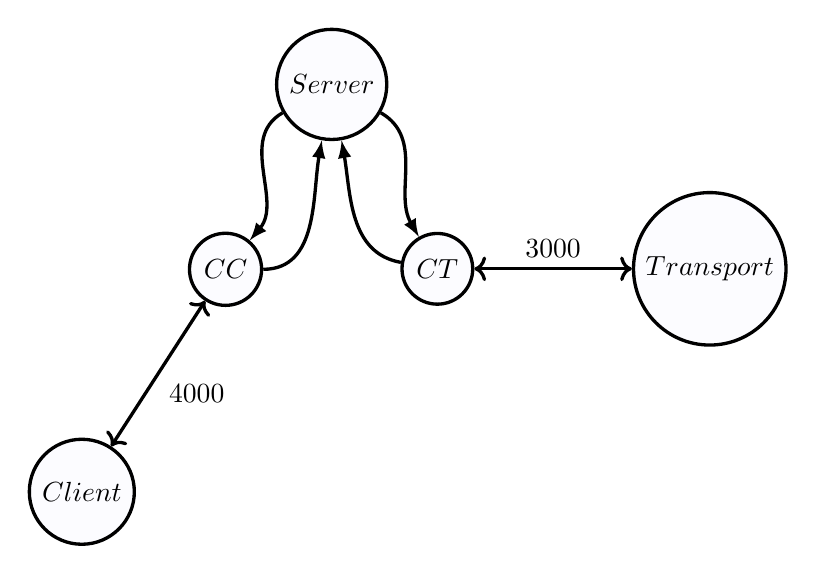
\begin{tikzpicture}[roundnode/.style={circle, draw=black!100, fill=blue!1, very thick, minimum size=5mm}] 
\node (2) [roundnode] {$Server$};
\node (3) [roundnode, below right=1.5cm and 0.5cm of 2] {$CT$};
\node (4) [roundnode, below left=1.5cm and 0.5cm of 2] {$CC$};
\node (5) [roundnode, below left=2cm and 1cm of 4] {$Client$};
\node (1) [roundnode, right=2cm and 2cm of 3] {$Transport$};
\draw [<->, very thick] (3) -- (1) node [midway, auto] () {3000};
\draw [<->, very thick] (4) -- (5) node [midway, auto] () {4000};
\draw [-latex, very thick] (4) to [out=0,in=-100] (2);
\draw [-latex, very thick] (2) to [out=-150,in=50] (4);
\draw [-latex, very thick] (3) to [out=-190,in=-80] (2);
\draw [-latex, very thick] (2) to [out=-30,in=120] (3);

\end{tikzpicture} 

Serverul principal isi va creea exact 2 copii care vor avea atributii diferite.\\
$1.$ $CC$ = $Child$ $Client$. Acesta se va ocupa de inregistrarea cerintelor clientului, transmiterea acestora catre server, precum si furnizarea raspunsului final catre client.\\
$2.$ $CT$ = $Child$ $Transport$, care se va ocupa de preluarea si stocarea informatiilor transmise de $Transport$, procesarea comenzii transmise de catre $Server$, precum si trimiterea raspunsului catre parinte.\\
\hspace*{4mm} De asemenea, $Transport$ va simula in $real-time$ detalii despre autobuze si tramvaie precum viteza, ruta, statia curenta, numarul de identificare, posibilitatea oferirii asistentei pentru persoanele cu dizabilitati, capacitatea, numarul actual de persoane, orientarea, etc, si le va trimite o data la 3 secunde catre $CT$. La fiecare iteratie, acestea se vor actualiza in sensul ca algoritmul va decide in mod aleatoriu daca respectivul mijloc de transport a ajuns in urmatoarea statie precum si cate persoane au coborat si urcat.\\
\hspace*{4mm} Totodata, $serverul$ va juca rol de intermediar intre cei 2 copii, intrucat acesta realizeaza singura conexiune intre procesele-fiu.\\
\hspace*{4mm} Dintr-un punct de vedere tehnic al implementarii, toata simularea se bazeaza pe comunicarea intre procese cu ajutorul unui socket conectat la port-ul $4000$ intre $client$ si $CC$, unui socket conectat la port-ul $3000$ intre $transport$ si $CT$ + 4 pipe-uri ce asigura fluxul de octeti intre $server$ si cei 2 copii. \\
\hspace*{4mm} Pentru evitarea caracterului blocant al apelului functiei $read()$ se va folosi functia $select()$ ce va monitoriza diferiti $file$ $descriptori$, in functie de proces. Astfel: \\
- $transport$ va monitoriza doar file descriptorul de citire aferent lui $CT$ \\
- $CT$ va monitoriza 2 file descriptori de citire: $transport$ si $server$ \\
- $server$ va monitoriza 2 file descriptori: $CC$ si $CT$\\
- $CC$ va monitoriza 2 file descriptori: $client$ si $server$\\
- $client$ nu va monitoriza nici un file descriptor, intrucat acesta doar trimite o comanda si asteapta in mod blocant raspunsul prin apelarea functiei $read()$.

\section{Detalii de implementare}
\subsection{Crearea socket-ului}
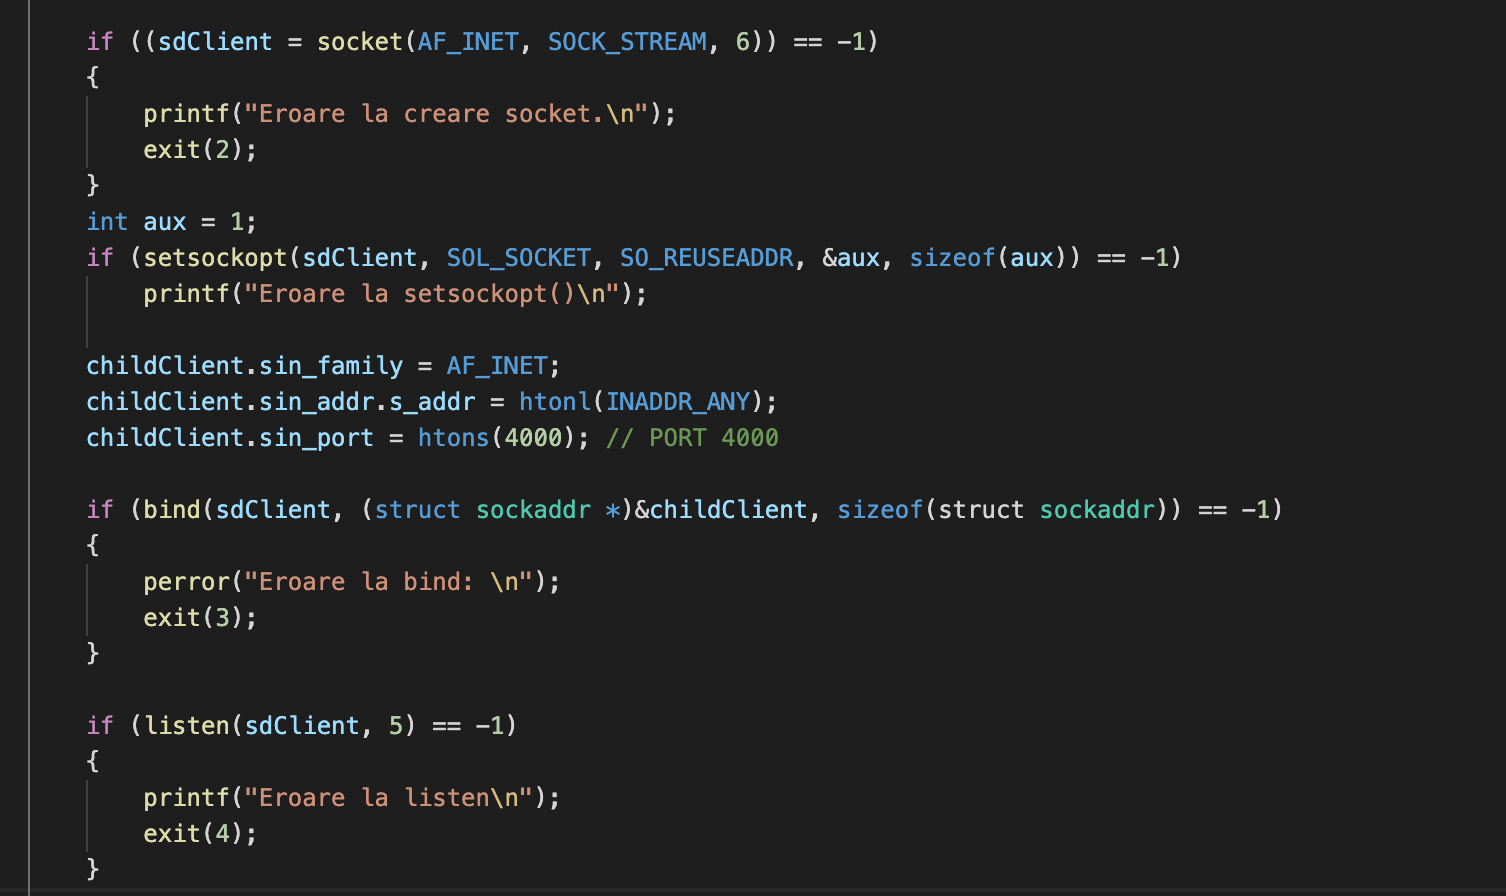
\includegraphics[scale=0.55]{socket}
\hspace*{4mm} Acest prim exemplu de implementare este preluat din codul scris in $CC$ si reprezinta crearea liniei de comunicatie cu clientul folosind un socket. In prima parte se poate observa folosirea protocolului $IPV4$ prin constanta $AF\_INET$, dar si folosirea unui $TCP$ prin constanta numerica $6.$ Adaugarea functiei $setsockopt()$ este optionala, aici fiind folosita pentru a-i comunica kernel-ului refolosirea portului daca acesta este ocupat. Dupa popularea structurii $childClient$ de tip $sockaddr\_in$, aceasta se leaga de file-descriptorul $sdClient$ ca apoi sa anuntam socket-ul ca poate accepta clienti prin $listen()$. \\
\vspace{10mm}
\subsection{Serializarea}
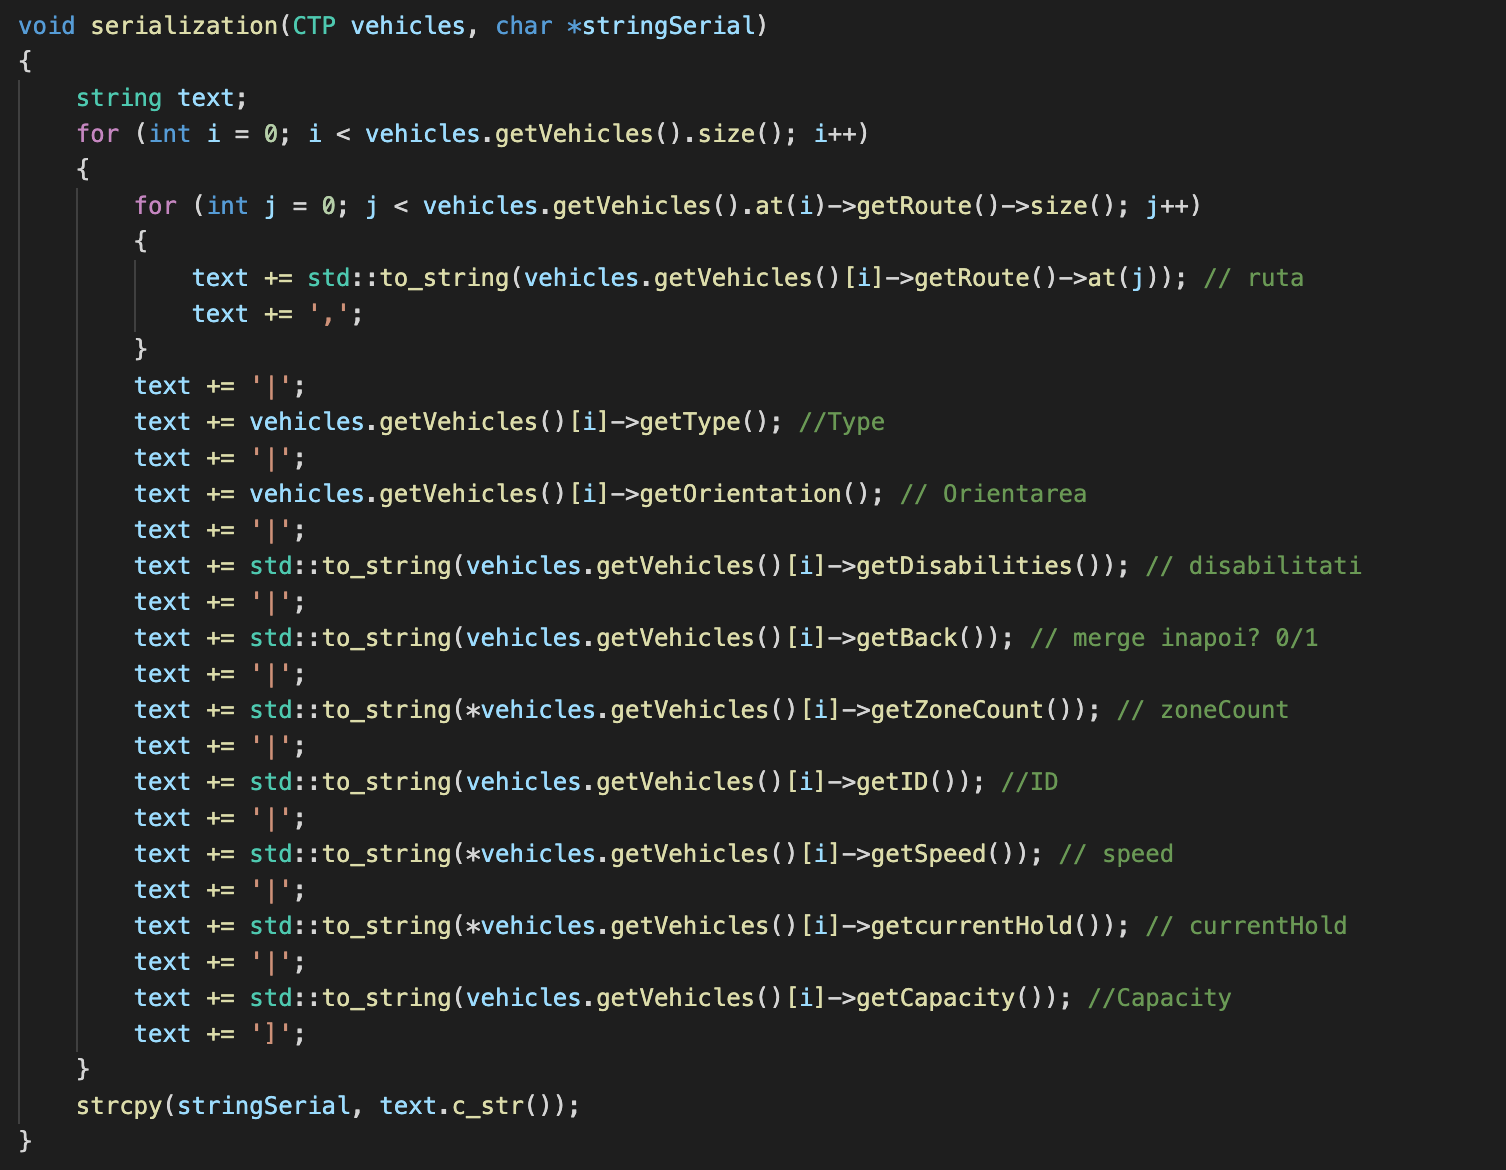
\includegraphics[scale=0.55]{serializare}
\hspace*{4mm} Un alt exemplu relevant pentru acest proiect ar fi serializarea informatiilor din procesul $transport$ pentru a putea fi transmise prin socket catre $CT$. Aceasta metoda este una favorabila din pricina timpului alocat executiei si a fiabilitatii. Avand in vedere ca prin socket nu se pot transmite pointeri la structuri intrucat acestia sunt locali masinii iar trimiterea unei intregi structuri este deseori evitata din pricina dificultatii de implementare, serializarea reprezinta o modalitate prin care putem codifica si salva cu usurinta starea curenta a mijloacelor de transport. Astfel, cu ajutorul unui $char*$, informatiile pot fi transmise printr-o simpla apelare a functiei $write()$. In cazul meu, dupa fiecare camp din structura va aparea caracterul $\vert$ pentru a putea deosebi trecerea de la un camp la altul, precum si ] pentru sfarsitul datelor despre un mijloc de transport.\\
\hspace*{4mm} Deserializarea este realizata pe "cealalta parte" a socket-ului. Se va citi acest sir de octeti intr-un $char[]$ iar apoi se va decodifica mesajul, populand o structura ce va avea aceleasi atribute.

\vspace{10mm}
\subsection{Functia $select()$}
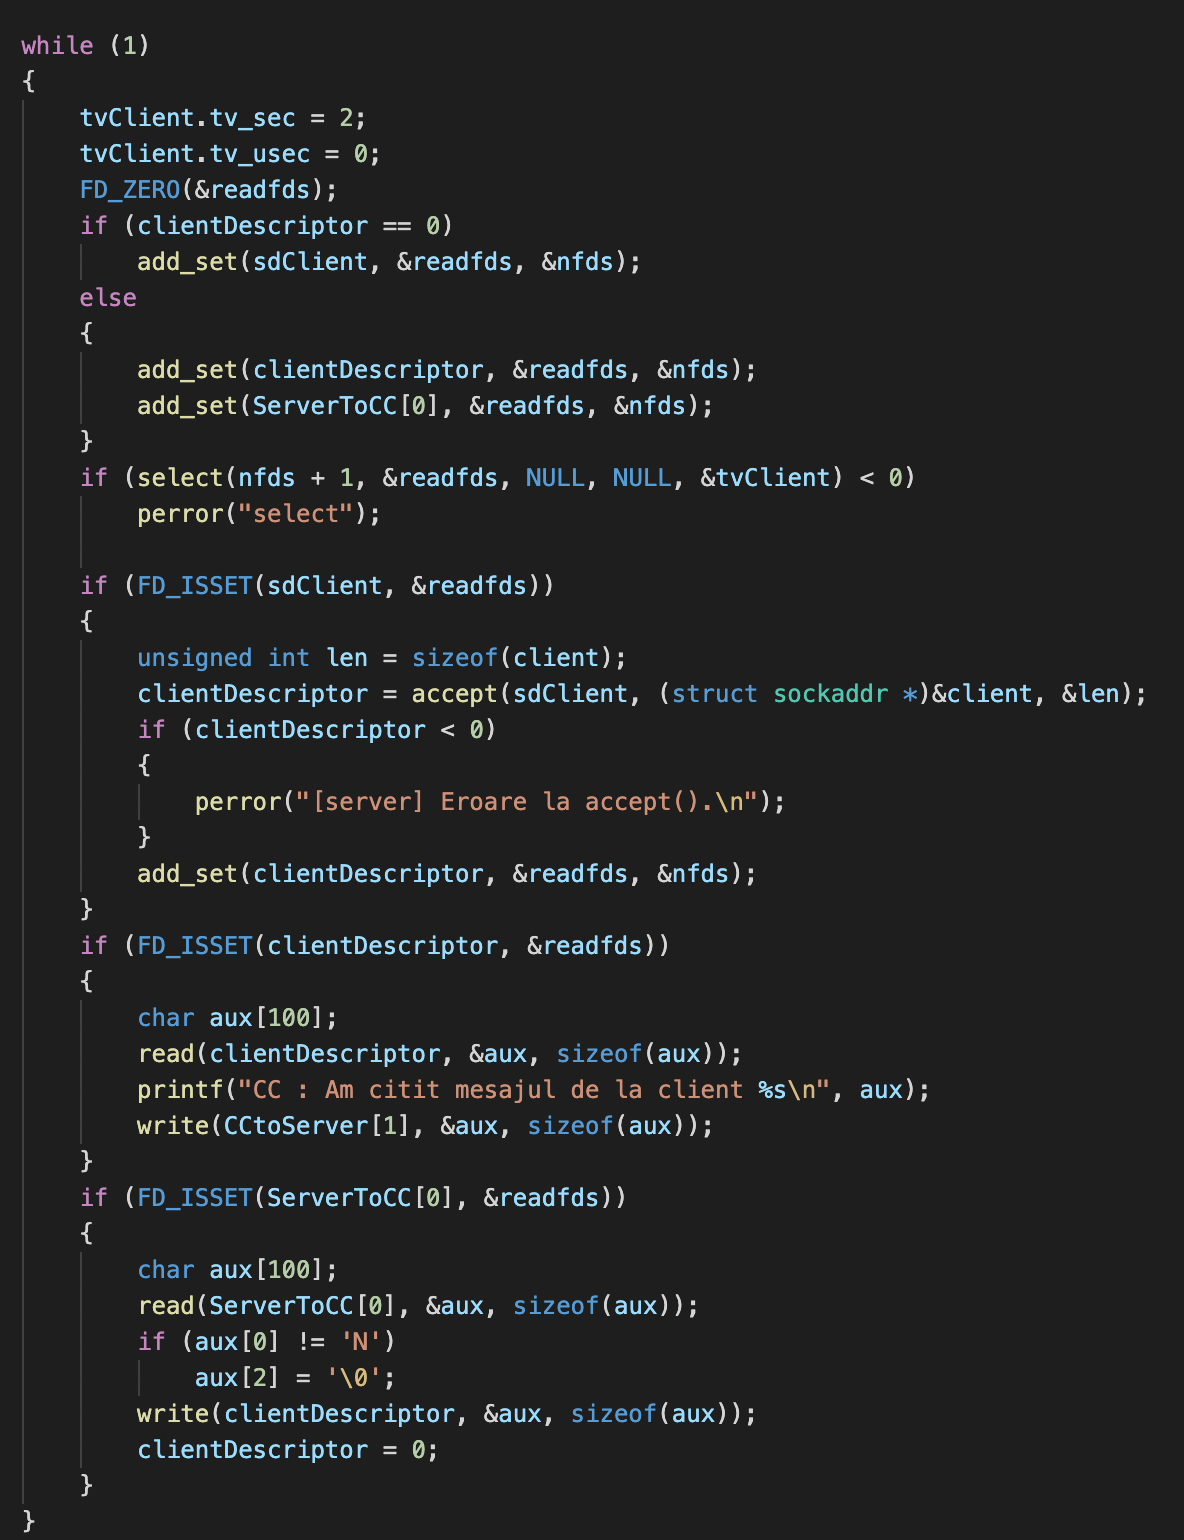
\includegraphics[scale=0.55]{select} \\
\hspace*{4mm} Inca o componenta principala a acestui proiect o reprezinta folosirea functiei $select()$ ce imi permite sa ascult mai multi file-descriptori pana cand unul devine $ready$. Am ales folosirea acestei functii deoarece am avut nevoie ca fiecare apel de $read()$ sa nu fie blocant $\Rightarrow$ citim din socket/pipe doar atunci cand sunt octeti disponibili. \\
\hspace*{4mm} Exemplul de mai sus este luat din codul scris in interiorul lui $CC$. Acesta verifica daca sunt octeti disponibili pentru citire din socket-ul catre client si pipe-ul catre server. Atunci cand unul dintre ei este disponibil, executa comenzile corespunzatoare de citire/scriere.

\vspace{4mm}

De asemenea, am incercat pe tot parcursul acestui proiect sa pastrez un caracter mai general al obiectelor. Astfel, urmatoarele aspecte sunt generate automat de catre algoritm: harta, traseele tuturor autobuzelor/tramvaielor, calibrarea hartii, a punctelor si a liniilor din grafica 2D. Programul trebuie doar sa stie numarul de noduri din graful ce va reprezenta harta (acesta trebuie sa fie patrat perfect). \\
\hspace*{4mm} Pentru implementarea unei interfete grafice 2D am folosit SFML prin care am reusit sa dinamizez ruta mijloacelor de transport. Atunci cand un client va solicita o informatie de la server, statia in care se afla clientul se va colora in verde pentru a observa mai usor functionalitatea algoritmului.

\section{Concluzii}
\hspace*{4mm} Solutia de rezolvare a problemei ar putea fi imbunatatita prin folosirea protocolului $UDP$ in loc de $TCP$ care favorizeaza timpul de transmitere a datelor in defavoarea fiabilitatii acestora. Pe langa posibilitatea de imbunatatire, exista si o probabilitate mare de aparitie a erorilor pe parcursul executarii programului deoarece unele datagrame se pot pierde $\Rightarrow$ informatiile pot fi eronate sau pot chiar lipsi. \\
\hspace*{4mm} De asemenea, pentru eficientizarea transmiterii datelor prin pipe-uri, putem configura serverul astfel incat acesta nici sa nu faca parte din procesarea datelor de la client. In aceasta situatie, ar fi nevoie de 2 pipe-uri in loc de 4 ce vor fi legate intre cei 2 fii.

\section{Bibliografie}
$1.$ https://en.wikipedia.org/wiki/IPv4  \\
$2.$ https://www.cloudflare.com/en-gb/learning/ddos/glossary/tcp-ip/ \\
$3.$ https://www.techopedia.com/definition/26184/c-plus-plus-programming-language


\end{document}
